\documentclass{beamer}
\setbeamertemplate{navigation symbols}{}
\usepackage{comment}

\setbeamercolor{frametitle}{fg=black,bg=white}
\setbeamercolor{title}{fg=black,bg=yellow!85!orange}
\usetheme{AnnArbor}

\usepackage{textpos} % package for the positioning
\usepackage{listings}
\usepackage{xcolor}
\usepackage[most]{tcolorbox}
\usepackage{mathtools}
\usepackage{graphicx}
\usepackage{graphbox}
\usepackage{movie15}
\usepackage{caption}
\DeclareCaptionType{code}[Code Listing][List of Code Listings] 

\definecolor{codegreen}{rgb}{0,0.6,0}
\definecolor{codegray}{rgb}{0.5,0.5,0.5}
\definecolor{codepurple}{rgb}{0.58,0,0.82}
\definecolor{backcolour}{rgb}{0.95,0.95,0.92} 
\lstdefinestyle{mystyle}{
    backgroundcolor=\color{backcolour},   
    commentstyle=\color{codegreen},
    keywordstyle=\color{magenta},
    numberstyle=\tiny\color{codegray},
    stringstyle=\color{codepurple},
    basicstyle=\ttfamily\footnotesize,
    breakatwhitespace=false,         
    breaklines=true,                 
    captionpos=b,                    
    keepspaces=true,                 
    numbers=left,                    
    numbersep=5pt,                  
    showspaces=false,                
    showstringspaces=false,
    showtabs=false,                  
    tabsize=2
}

\lstset{style=mystyle}

\lstdefinelanguage
   [x64]{Assembler}     % add a "x64" dialect of Assembler
   [x86masm]{Assembler} % based on the "x86masm" dialect
   % with these extra keywords:
   {morekeywords={CDQE,CQO,CMPSQ,CMPXCHG16B,JRCXZ,LODSQ,MOVSXD, %
                  POPFQ,PUSHFQ,SCASQ,STOSQ,IRETQ,RDTSCP,SWAPGS, %
                  rax,rdx,rcx,rbx,rsi,rdi,rsp,rbp, %
                  r8,r8d,r8w,r8b,r9,r9d,r9w,r9b, %
                  r10,r10d,r10w,r10b,r11,r11d,r11w,r11b, %
                  r12,r12d,r12w,r12b,r13,r13d,r13w,r13b, %
                  r14,r14d,r14w,r14b,r15,r15d,r15w,r15b}} %


\beamersetuncovermixins{\opaqueness<1>{25}}{\opaqueness<2->{15}}

%Copyright
\addtobeamertemplate{frametitle}{}{%
\begin{textblock*}{50mm}(0cm,-1.25cm)
\color{yellow!85!orange}
\tiny{Copyright \copyright 2024 CNM.}
\end{textblock*}}

% position the logo
\addtobeamertemplate{frametitle}{}{%
\begin{textblock*}{100mm}(11.4cm,-1.3cm)

\includegraphics[height=1cm,width=1cm,keepaspectratio]{fig/ddclogotransparent.png}
\end{textblock*}}

\AtBeginSection[]{
  \begin{frame}
  \vfill
  \centering
  \begin{beamercolorbox}[sep=8pt,center,shadow=true,rounded=true]{title}
    \usebeamerfont{title}\insertsectionhead\par%
  \end{beamercolorbox}
  \vfill
  \end{frame}
}

\begin{document}
\title{Quantum Technician Bootcamp}
\author{Brian Rashap}
\date{September 2025} 

\begin{frame}
\titlepage
\end{frame}

\section{Safety}

\begin{frame}\frametitle{Safety Walk}
\begin{center}
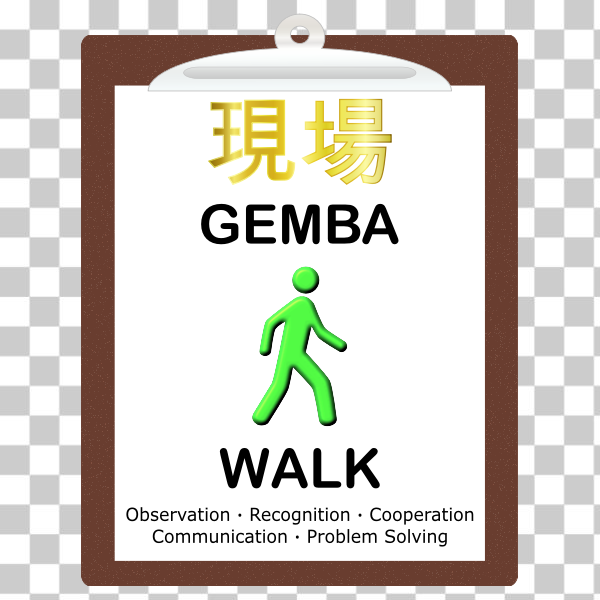
\includegraphics[width=6cm]{fig/gemba.png}
\end{center}
\end{frame}

\begin{frame}\frametitle{Laser Safety - Laser Classes}
\begin{center}
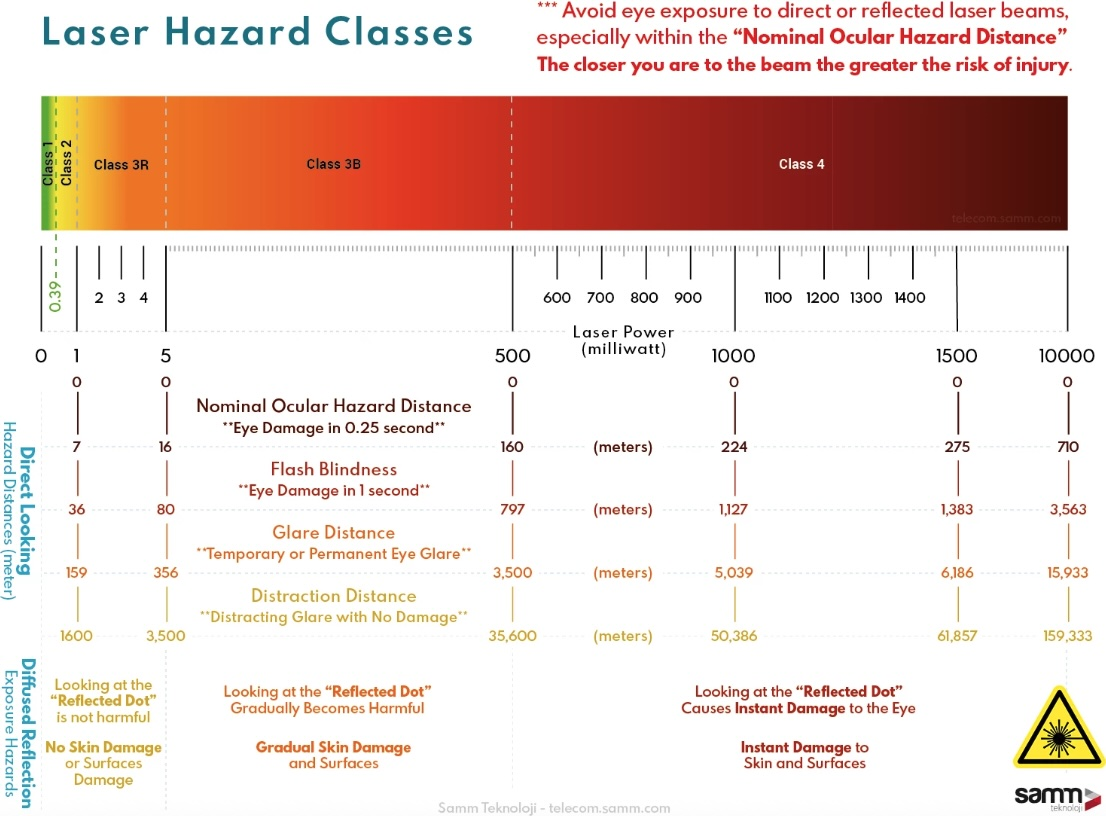
\includegraphics[width=10cm]{fig/lasersafe.jpg}
\end{center}
\end{frame}

\begin{frame}\frametitle{Laser Safety - Class 2}
\begin{center}
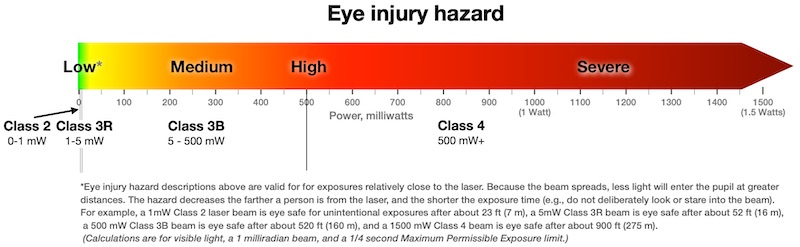
\includegraphics[width=10cm]{fig/lsafe.png}
\end{center}
\begin{itemize}
\item Class 2 lasers, which are limited to 1 mW of visible continuous-wave radiation, are safe because the blink reflex will limit the exposure in the eye to 0.25 seconds. This category only applies to visible radiation (400 - 700 nm).
\end{itemize}
\end{frame}

\begin{frame}\frametitle{Laser Safety - Class 3R}
\begin{center}
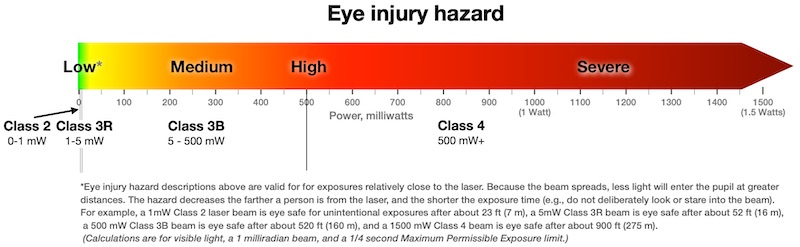
\includegraphics[width=10cm]{fig/lsafe.png}
\end{center}
\begin{itemize}
\item Class 3R lasers produce visible and invisible light that is hazardous under direct and specular-reflection viewing conditions. Eye injuries may occur if you directly view the beam, especially when using optical instruments. Lasers in this class are considered safe as long as they are handled with restricted beam viewing. Visible, continuous-wave lasers in this class are limited to 5 mW of output power.
\end{itemize}
\end{frame}

\begin{frame}\frametitle{Laser Safety - Class 3R}
\begin{center}
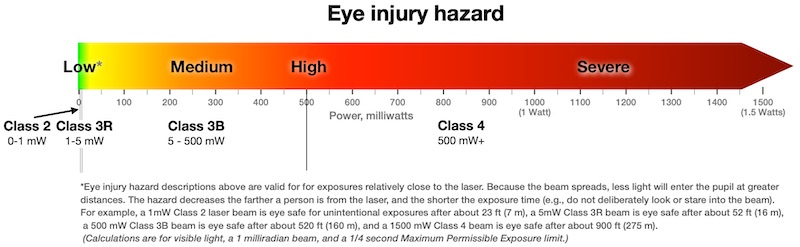
\includegraphics[width=10cm]{fig/lsafe.png}
\end{center}
\begin{itemize}
\item Class 3B lasers are hazardous to the eye if exposed directly. Diffuse reflections are usually not harmful. Safe handling of devices in this class includes wearing protective eyewear where direct viewing of the laser beam may occur. Lasers of this class must be equipped with a key switch, laser safety signs should be used. Laser products with power output near the upper range of Class 3B may also cause skin burns.
\end{itemize}
\end{frame}

\begin{frame}\frametitle{Lock Out Tag Out}
\begin{center}
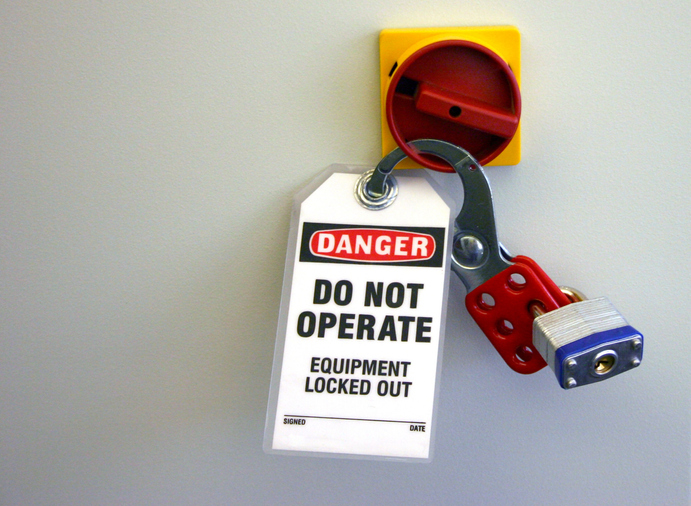
\includegraphics[width=4cm]{fig/loto.jpg}
\end{center}

\begin{itemize}
\item Electrical Energy
\item Mechanical Energy
\item Mechanical Energy - Pneumatics
\end{itemize}
\end{frame}

\begin{frame}\frametitle{Sharps}
\begin{center}
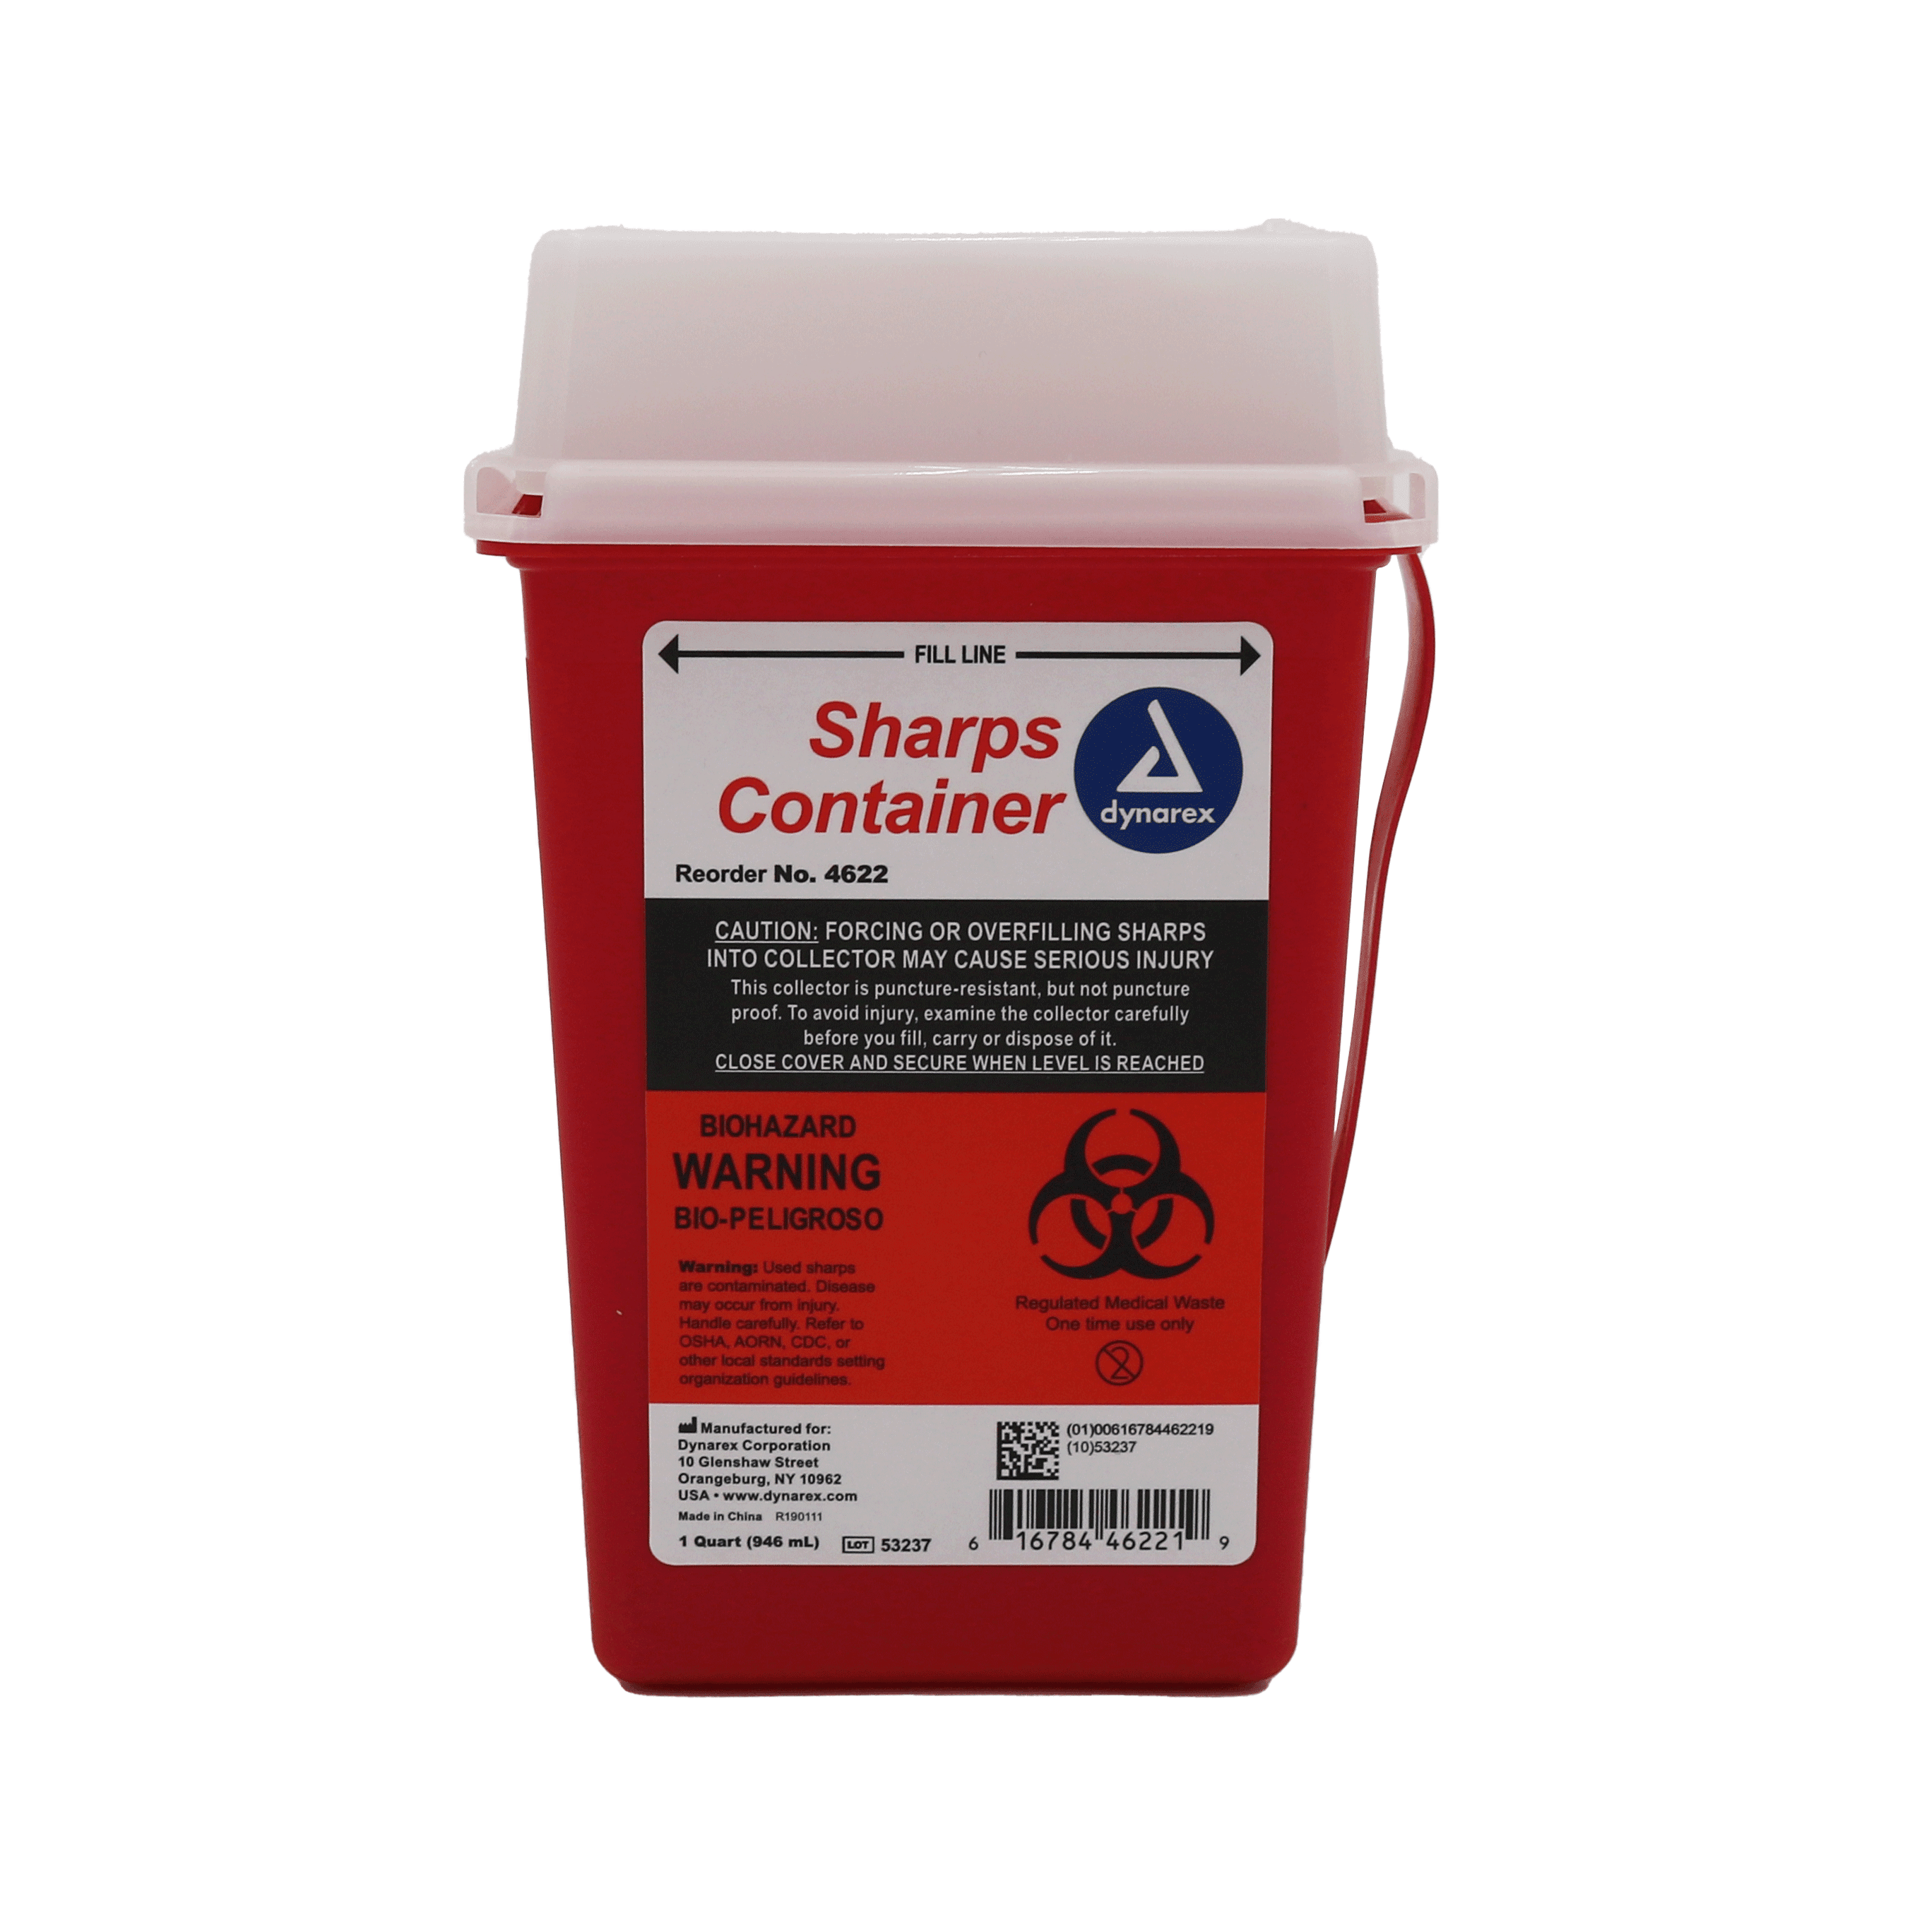
\includegraphics[width=6cm]{fig/sharps.png}
\end{center}
\end{frame}


\begin{frame}\frametitle{High Voltage}
\begin{center}
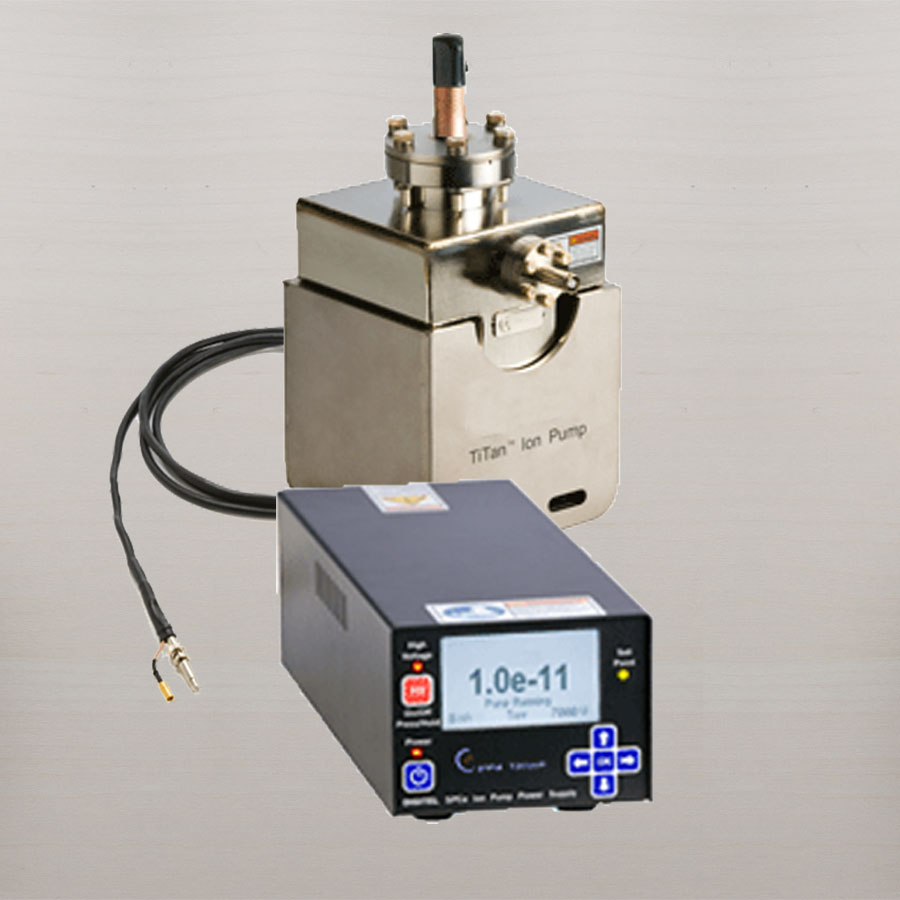
\includegraphics[width=6cm]{fig/highV.jpg}
\end{center}
\end{frame}




\end{document}
